\section{From ownership to executed development}
\label{sec:development}

\subsection{Construction access and response resolution}

All sixty-three trade-completed groups reach a first management window, and forty-three receive construction. Sol builds on sixteen of seventeen, Gemini seventeen of eighteen, Opus seven of fifteen and Grok three of thirteen. The twenty unbuilt groups comprise nine for which no recorded menu offers construction on that group, four defaults, four received-call conflicts and three other valid ends (Figure~\ref{fig:execution}). Grok's ten comprise four group-specific no-option windows with stated financing deferrals, four conflicts and two stated holds. Opus's eight comprise five group-specific no-option windows under action-only recovery and three defaults. Sol's single unbuilt group ends in a default; Gemini's ends with a valid turn-ending action.

\begin{figure}[t]
\centering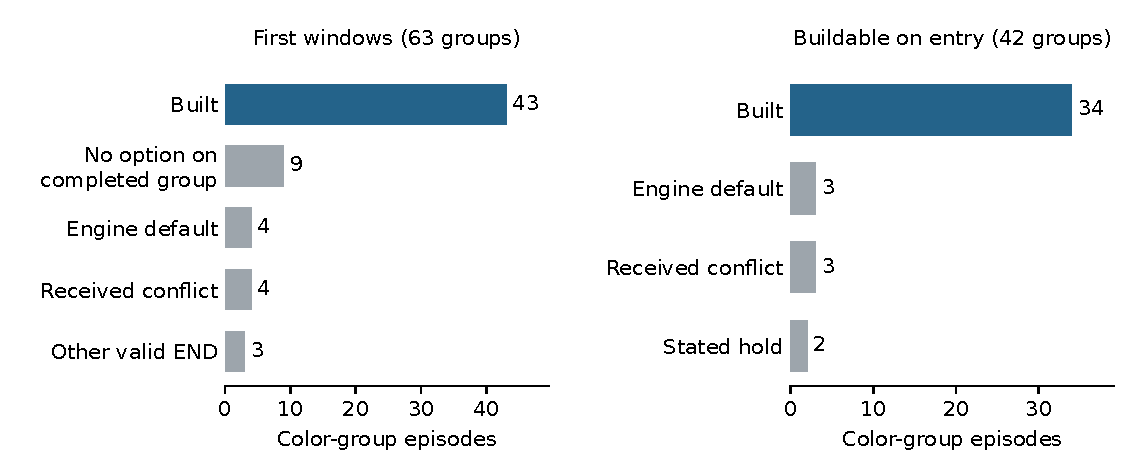
\includegraphics[width=\linewidth]{execution.pdf}
\caption{Development after trade completion. The whole-window population contains 63 groups; the subset buildable on entry contains 42. Availability is measured for the newly completed group. Two G1 no-option windows offer construction on a different group. A received conflict denotes disagreement between content and call, not a validated alternative plan.}
\label{fig:execution}
\end{figure}

Seven of the nine no-option groups receive a mortgaged completing deed. Another, Opus's G20 dark blues, already contains a mortgaged Boardwalk; only Opus's G15 dark blues have no mortgage but insufficient cash for a house. Static budgets at the first post-completion management decision show that two owners can cover redemption and a house with cash alone: Grok has \$602 against \$193 plus \$200 in G14, and \$523 against \$111 plus \$100 in G16. Counting currently mortgageable deeds outside the target group supplies the budget in five more cases. The remaining two fall short of this mortgage-only budget. Bank houses are available in all nine.

The budgets distinguish immediate access from financing choices (Appendix~\ref{app:access}). All four Grok notes explicitly defer redemption or construction to preserve liquidity. In its two G1 windows, the menu also offers an Atlantic house on the already-owned yellow group; Grok declines that investment too. G16 Opus redeems Park Place and ends with \$75 while two other deeds remain mortgageable. Thus a newly completed group can remain undeveloped because its owner preserves cash or collateral elsewhere, even when a static financing budget is sufficient.

Among the forty-two groups buildable on entry, thirty-four receive construction. The eight residuals comprise three defaults, three conflicts and two stated holds. Financing can also precede a conflict: Grok mortgages deeds before its G8, G12 and G13 build-requesting responses end the turn instead. The G8 and G13 content names one-house-per-deed plans consistent with the displayed cash, stock and target keys; the G12 3/2/2 encoding would fail per-entry evenness. G20's content names a mortgage. These plans were not newly executed for this study, but the records distinguish attempted investment from a stated choice to wait.

The broader record contains 663 applied \End{} actions on management menus offering construction somewhere. Sixty-six are defaults and twenty-four are content/call conflicts; in twenty-two of those conflicts the content names construction. Appendix~\ref{app:conditions} retains this accounting separately from the group-level windows.

\subsection{Construction requests, recovery and reserve choices}

All sixty-one defaulted Opus construction purchase multisets execute in the retained historical checks after count-valued entries are split and purchases legally interleaved. Cash, stock and requested purchases are unchanged. The submitted plans remain invalid. Sixty chains have a provider refusal followed by invalid action-only construction; G2 d129 has invalid construction followed by refusal. In both orders the response budget is exhausted and the engine ends management.

Other configurations often recover a rejected construction request. Among uneven-build rejections ending in construction, the original purchase multiset is preserved in 20/25 Sol, 6/18 Gemini and 5/5 Grok decisions. A changed allocation can also be a successful correction. G14 d145--148 realizes an initial eight-house target over several management decisions even though its first correction does not preserve that target. Appendix~\ref{app:validation} gives the full target and default accounting.

Reserve choices are also explicit. At G3 d176, Opus ends with \$204 and its action-only assistant content prefers retaining cash to buying an available \$150 house. At G1 d426, Grok declines another yellow house with \$488, citing its financing needs. These are expressed choices to retain liquidity, distinct from requested builds that the response path does not execute.

\subsection{Realized receipts and a rival's construction budget}

Trade-completed groups receive \$57,378 in rent from completion until loss or game end. The forty-three groups built on in the first window collect \$53,810; the twenty others collect \$3,568, and eleven of those are built on later. Early development and later receipts therefore occur together in this corpus. These are total paid receipts, including undeveloped rent, under differing exposure and survival times. Appendix~\ref{app:economy} gives the per-configuration totals.

Across the 103 game/player/group spending units, construction outlay is \$103,450 and whole-game paid developed rent is \$93,000. Forty receive no developed rent, although some still trigger a creditor elimination. The distinction matters economically: a rent demand can transfer an estate rather than appear as a cash receipt. Salvage, inherited buildings and terminal unpaid debts are accounted for separately in Appendix~\ref{app:economy}.

\TranscriptTitle{g20}{An appeal to withhold a rival's building cash}

In G20, Opus sells Illinois to Grok for \$500, completing reds and leaving Grok \$222. A red house costs \$150. Gemini addresses the table:
\TranscriptQuote{g20-coordination-appeal}
Grok's next note recognizes the appeal:
\TranscriptQuote{g20-recognition-note}
That decision's received call ends management while its content requests a mortgage. After later construction, Grok tries to sell Vermont to Gemini for \$150. Gemini replies:
\TranscriptQuote{g20-concrete-refusal}
\TranscriptFinding{Grok mortgages Vermont for \$50 instead. Opus later makes two cash offers for Grok's property; neither settles. Gemini wins.}
\TranscriptReading{Gemini explicitly asks others to deny a rival construction funds, Grok recognizes the appeal, and Gemini follows through when offered a purchase. Sol had already recorded its own financing objection privately at d95. Opus later offers cash expressly for Grok's house funding, but Grok rejects or counters those bids. The observed coordination is therefore an appeal and its author's follow-through, not a jointly adopted cartel.}
\TranscriptSource{G20 d95--102, d129--130 and d156--160. The appeal is in Grok's d97 request. The quoted note belongs to selected attempt 1 after a malformed first attempt.}
\FloatBarrier
